\section{The centralised state of the world}
How we communicate, how we buy and sell goods and services and even how we store our valuable information, is centrally controlled and manipulated. Almost two-thirds of the internet’s data is stored and processed on servers owned and controlled by just four global institutions. Three companies control the distribution of apps - and their resulting revenue streams - on almost every one of the world’s three billion smartphones and homepods. Over the past 5 years, Google and Facebook alone have crept from managing 50\% of the traffic to top web publishers, to 75\% today.
The problems with centralised growth cycles are well known. When they start out, they do everything they can to grow their network and recruit users and other important ecosystem members like developers and businesses. Sadly, however, when centralised platforms reach a certain scale, their relationships with network participants change from positive-sum to zero-sum. As the concentration of power increases, the “mistakes” of these power players trigger greater and greater harms, the magnitude of which is unprecedented. Unfortunately, by this stage, people are so dependant on these big players that they become apathetic. 
Centralised platforms’ consistent dominance, has drawn people into forgetting they have a choice. There is a better way to build internet services. We have that choice. Why a decentralised system is so necessary - as opposed to a centralised system - is that scale makes the system more resilient. None of the nodes are central. None are essential. There is no single point of failure. 
The value of decentralised systems was first seen in the early days of the internet. The Ki Foundation is working to ensure that we’ll get to see that value again in the next wave of the internet. The Ki ecosystem will use multiple mechanisms to avoid problems associated with centralised platforms. First, the project will be fully open source. Second, in the Ki network, important governance decisions will be made by the community, using open and transparent practises. As we know from the offline and political worlds, democratic systems aren’t perfect, but they are a lot better than the alternative. 
We are at a point in our history as humans, where it is no longer just the global open source and blockchain communities yearning for a fairer, more transparent and correctly incentivised infrastructure to make a decentralised, safer and more equitable world. We all need a better solution. 

\section{The dangers related to the Internet of Things (IOT)}
The IoT market has exploded in the last few years, boosted by a new generation of closed and heterogeneous technologies and services, such as Z-Wave, Zigbee, LORA, Wi-Fi, Bluetooth, Home Connect, etc. As a result, we have seen the rise of homepod devices like Amazon’s Alexa™ or Google Home™, which have emerged as the dominant hubs for smart home connected hardware. The current homepod offerings are cloud-based, with their core principles and modus operandi being to continuously record, eavesdrop and commoditize users’ personal data. We now live in an era with surveillance capitalism in a symbiotic relationship with advertising technology. This very model is, by design, a threat to the privacy of individuals within their home. As control of more and more user data continues to empower the technology giants, it also provides a global surveillance platform for the world’s governments, which may eventually become too tempting not to compromise. 
This accumulation of data is, in and of itself, not a personal privacy issue, but a massive public security problem. If privacy becomes a commodity, one that only the rich can afford, then the rich can and will use this information asymmetry to threaten and persecute people who challenge the status quo, thereby perpetuating it. The world is starting to pay attention to issues pertaining to central server storage of their personal information. Decentralized storage, as evidenced by projects like the Interplanetary File System, Filecoin, Storj, and Maidsafe, present the best possible way to avoid the pitfalls of centralized data silos while not sacrificing increasingly important values like user privacy, access to information, and security. More hacks of centralized servers are on the way. As this problem grows into an epidemic with very real consequences for everyday people, users and companies will look to blockchain and distributed storage solutions for an answer. 
In the face of this age of surveillance capitalism, we propose an alternative solution to this dystopian future. We propose a future in which users can take back ownership of their personal data, a future in which users have privacy within their own homes.

\section{The Ki Foundation’s mission}

Ki is creating a new digital, connected home, built on a decentralised internet and the principles of privacy, security and the fair sharing of value. The Ki Foundation wants to change the current status quo whereby you, as a citizen of the internet, must relinquish all control of your data and privacy in order to access essential internet services. The Ki ecosystem will not rely on monetising users personal data and can therefore enforce a privacy-centric approach to technology, preserving its users’ privacy.

\section{Ki Blockchain: The next-gen blockchain for the IoT}
\label{ch1}
Ki is building a new decentralised ecosystem, which will provide users with access to a vibrant and open ecosystem of applications and services, without forcing them to relinquish control of their data. The Ki Foundation’s objectives for this new ecosystem focuses on the fair sharing of value. This enables two key things: 1) an open development ecosystem and decentralised marketplace for dApps, and 2) a new resource sharing paradigm, where, anything with computational power, storage and connectivity can be monetised and leased in real-time, with minimal effort from both the resource providers and the users. Utilising Ki's new Proof of Reputation consensus mechanism and scalable new blockchain, control the governance of the Ki ecosystem and the value arising from it, will be shared across all of the network’s participants.
Ki’s ambition is to become the standard for the valuation of any service offered by anything powered by a chip and connected to a network or a sub network. Using Ki, any hardware, even with very little processing power or no data-storage should be able to monetise its resources. The end vision is to secure and fairly distribute the world's data, starting with the privacy of hotels and homes, then decentralising data processing and storage and finally, unlocking energy ecosystems around the world.
The Ki Foundation is working to build a new scalable and secure blockchain protocol that can deal with thousands of transactions per second using very low computational power - without sacrificing on the organisation’s ethos of fairness and commitment to decentralisation. A further design consideration of the Ki Blockchain is to have full Solidity support in order to onboard most of the existing dApps and developers working on different chains.
\subsection{Why a new Blockchain?}
All existing consensus protocols raise some issues related either to energy efficiency, performance, robustness, privacy, or attack resistance. In a nutshell, these drawbacks can be summarized as follows: the Proof of Work (PoW) consensus protocol is unfair as the validation power is correlated to the expensive computational capacity dominated by the professional validators and the large pools. Moreover, it has an important ecological footprint and is insecure for small networks (consequently, every network at launch). On its side, the Proof of Stake (PoS) consensus protocol is also unfair as the validation power is correlated to the validators' wealth. Besides, it is vulnerable to nothing in stake attacks and suffers from a scalability issue. The Delegated Proof of Stake (DPoS) consensus protocol solves the majority of these problems thanks to its delegation process. In DPoS Users (a.k.a. delegators) vote to select witnesses (a.k.a. delegates), witnesses who have collected the most votes access the rounds to validate transactions. Votes are weighted according to the size of each voters stake. A user does not need to have a large stake to be elected as a validator (like in PoS). Rather, votes from users with large stakes can result in users with relatively small stakes being elevated to the top tier of witnesses. Indeed, if the same witnesses are selected in each round, the validation process tends to become centralised, which compromises the integrity of the network and reduces the interests and incentive of new validators. Practically, many DPoS based blockchains have converged over the time to a quasi-fixed delegate list.
Based on this discussion, we summarize the goals of the novel blockchain we are proposing in 3 points:

\subsubsection{Incentivizing the validators} As mentioned earlier, one common drawback of PoW, PoS and DPoS is the practical obstacles preventing new validators from competing on block validation and on token creation. Indeed, this creates two problems: first, the network tends to be more and more centralized. This is contradictory to the conception of blockchain and of decentralized systems. A blockchain where the block validation power is detained by a fixed set of validators is vulnerable and insecure. Its vulnerability is correlated to the vulnerability of the validators (i.e. if the infrastructure of one or many of these validators is attacked, the blockchain integrity might be compromised ) and its security depends on their honesty and behavior. Second, the system tends to become unfair. That is, the wealthy gets wealthier and the voted validators becomes the hostages of their voters. Incentivizing new validators to access the validation process is vital for the network and essential for its security and fairness. Therefore we formalize our first objective of proposing the new PoR consensus protocol as follows:\\

\textit{The proposed blockchain aims at allowing an easier access to the validation process in order to incentivise new validators in joining the network.}

\subsubsection{Less tradeoff} The rationale behind setting a fixed set of validators in the DPoS consensus protocol is to ensure that reliability of the validators and avoid the nothing-at-stake problem through the community election and approval step. The problem rises when this community approval steps, which is essential to secure the networks starts laying always the same list of validators. That is equivalent to say that the security of the network becomes tightly linked to the centralization of the validation process. Again, this is indeed contradictory to the decentralization and fairness promises of blockchain. Therefore, we formalize our second objective of proposing the PoR as follows:\\

\textit{The proposed blockchain aims at allowing a looser correlation between the centralization of the validation process and the security of the blockchain. }

\subsubsection{Rationalizing liquidity} One problem of the DPoS protocol is that it allows delegators to trade and spend their delegated stakes. This is unnatural as one must not be able to use the same tokens twice, even when this doesn't mean that the token is double spent. Therefore, we formalize our third objective of proposing th PoR as follows:\\

\textit{The proposed blockchain aims at rationalizing the liquidity by differentiating staked tokens from usable tokens. }

\subsection{Building a fair, secure and scalable blockchain}
To fulfill the goals mentioned in the previous section, the Ki team, in partnership with the renowned French-based research laboratory, LIRIS, has been working on a new kind of consensus mechanism, called Proof of Reputation (PoR). This new consensus algorithm operates to allow an easier access to the validation process to increase the interest of new validators in joining the network. In order to guarantee the security of the blockchain while maintaining this easy access, Ki proposes a set of theoretical and practical measures. These points are explained hereafter.

\subsubsection{The Validator List}
As mentioned above, limiting the number of validators by a set of chosen ones becomes a threat to the security and the equity of the blockchain. Our solution to this limitation is to permanently change this list of validators and to randomly pick, among the eligible validators, a new set of an equal size at each round. Indeed, when talking about a random picking of the validator list, one needs to give theoretical guarantees about the likelihood that the selected set does not present a majority of potentially colluding validators. The higher the number of validators in each round is, the lower are the chances to pick enough colluding nodes. However, this renders the validation round longer, and thus validators must wait longer in order to get the chance to validate blocks. Indeed, the higher the confidence is in the potential validators, the lower the collusion probability gets. Hence a lower number of validators can be selected in each round.\\

\textit{Continuously renewing the validator list through a random selection process ensures the permanent decentralization of the validation power and a higher incentive for smaller validators.}

\subsubsection{Validator Reputation} From the previous subsection, one can derive an important aspect of the solution. That is, the eligibility metric. In PoS and DPoS systems, a selection metric i.e., the stake and the delegated stake respectively, is used to select the validators. This metric is deterministic and thus, it does not allow any degree of freedom when selecting the validator list, which in turns leads to the centralisation problem. The Ki Blockchain’s PoR consensus algorithm proposes to use an eligibility metric, which as stated before, allows the election of all of the reliable enough validators, among whom the validator set is selected randomly. In this work, we call this eligibility metric The Reputation. This approach raises multiple challenges. One being to define what a reliable validator is To answer this challenge we propose to set a list of behaviors that defines good and bad wallet and validator conduct. In a first iteration,    this list will contain common well known behaviors such as: invalid height, timeout, high latency, forks, too many requests, repeat offender and no common block. Then, we are planning to extend this list by nondestructively probing the network and identifying new behaviors that may be specific to our ecosystem. These behaviors can be used to build a profile for each validator, from which a reputation metric can be computed. 
This reputation metric constitutes the second challenge which can be expressed by the following question "how can the behaviour profile of the validator be translated to a low level numerical value?". In other words, suppose that for each validator we build a behaviour profile expressed as a binary vector where 0 means a bad behaviour and 1 means a good behaviour. To be able to rank validators, one needs a function that translate this 01 vector into a float based on which ranking is made. Basic way to do it: count the 1s in the vector. the higher the number is the more reliable the validator is. This, however, supposes all behaviours are equally important which is not realistic. A weighted sum of the 1s can be better. Now, in reality, behaviours can be binary features categorial features and numerical (continuous and discrete) valued features. One needs to find a way to combine all of them in one float. Indeed, the difficult part is more related to finding the weights and the granularity of the features and not really the aggregation function it self. The reputation based validation process is shown in Figure \ref{fig:wf}. 

\begin{figure}
	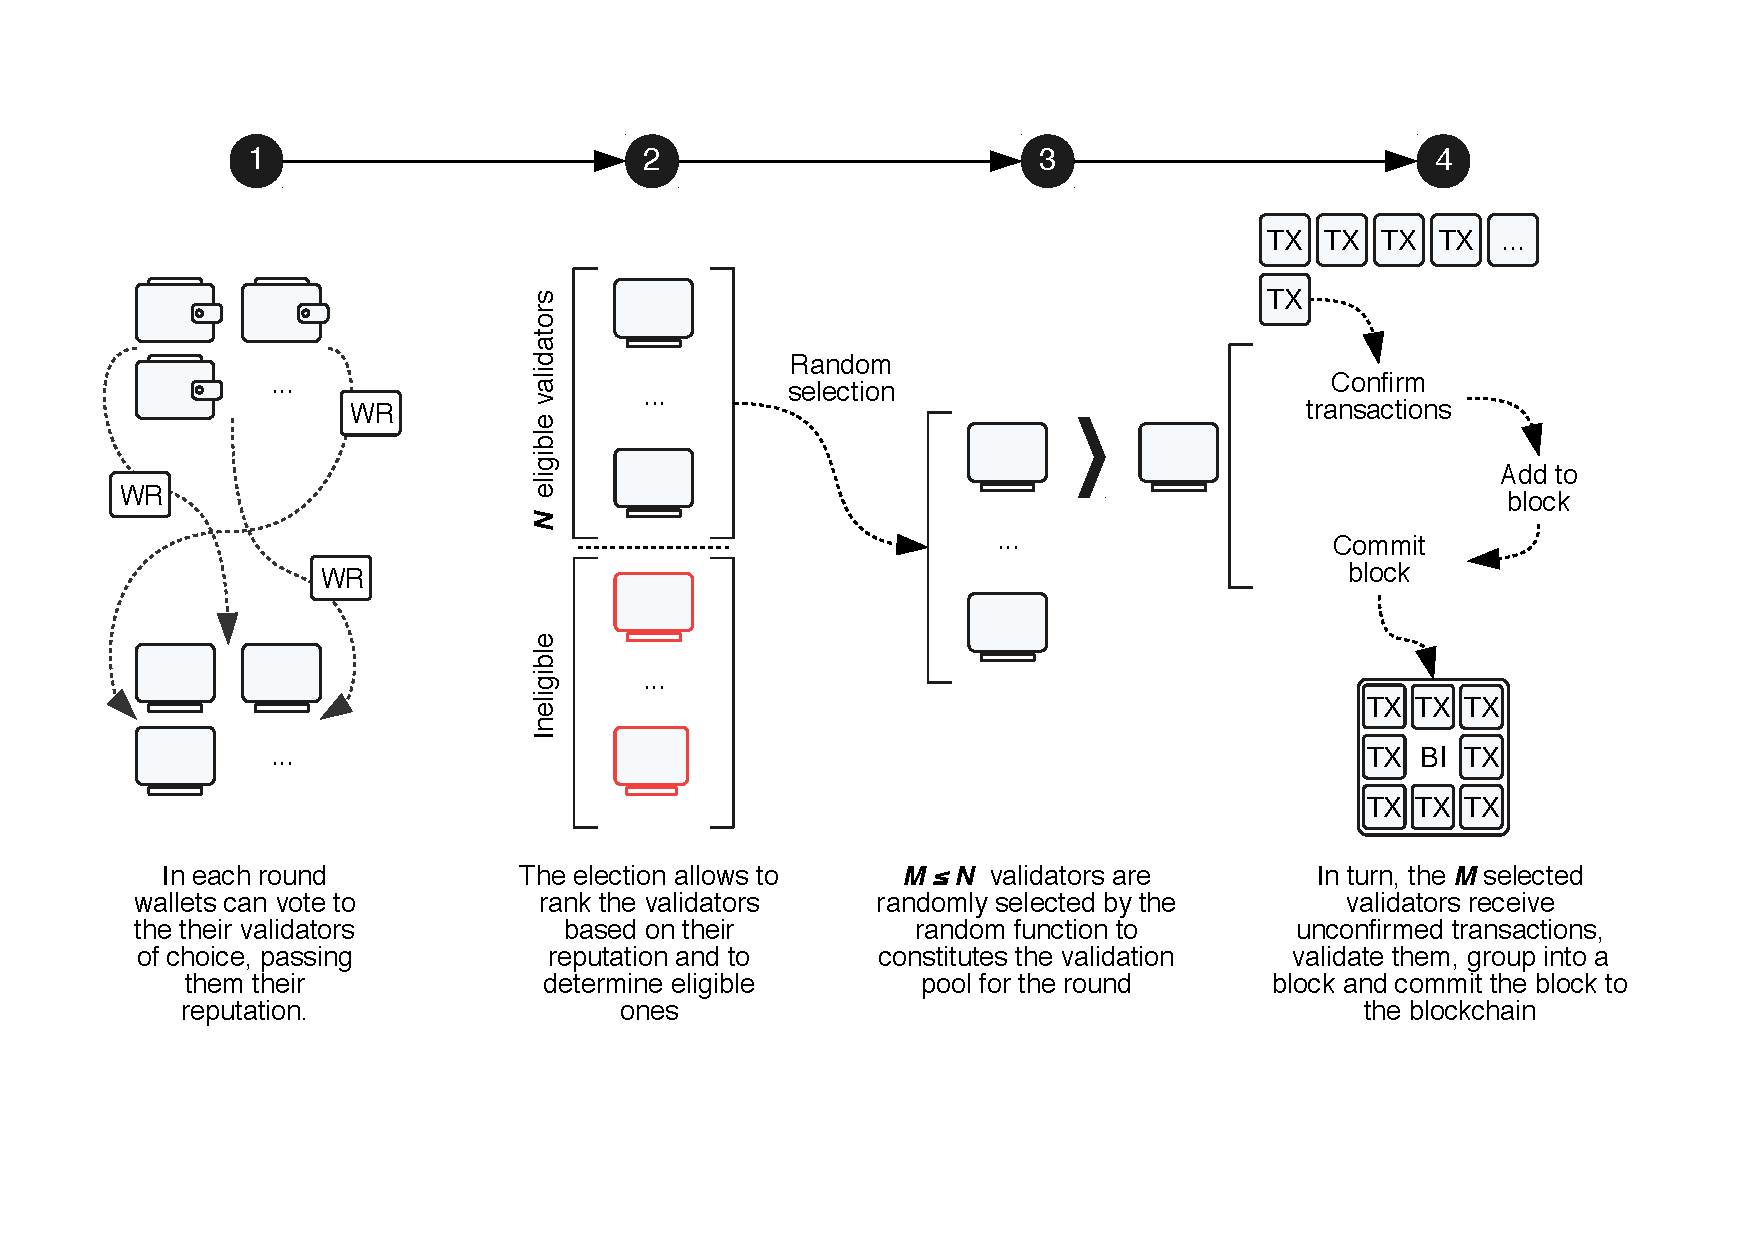
\includegraphics[width=\linewidth, trim= 1cm 3cm 1cm 2cm, clip]{Figures/workflow.pdf}
	\caption{An overview of the block validation workflow in the Ki Blockchain.}
	\label{fig:wf}
\end{figure}

This computation must fulfill the following requirements:
\begin{itemize}
	\item It needs to punish malicious behaviors.
	\item It needs to penalise negative contributions.
	\item It needs to incentivise positive contributions.
	\item It needs to be normalised so that it can be distributed and not centralised.
\end{itemize}

\textit{Determining the eligibility of the validators based on a behaviour dependent reputation score in addition to their stake guarantees the reliability of the validation process despite the random selection process of the validators.}

\subsubsection{Hot and cold wallets} In order to optimize the liquidity we start by differentiating between the current tokens and the staked ones. Concretely, we propose to endow each wallet with two subwallets: The current wallet and cold wallet. While the former contains tokens that can be traded and used to pay services, the latter contains tokens that have been staked upon voting for a validator. Token contained in the cold wallet can be even more valued, from the wallet reputation perspective, according to their coin age. That is the time during which they have been staked. The longer the coin have been staked the larger their weight is in the reputation of the wallet. The structure and attributes of the wallets in the Ki blockchain are shown in Figure \ref{fig:wallets}.  \\

\begin{figure}
	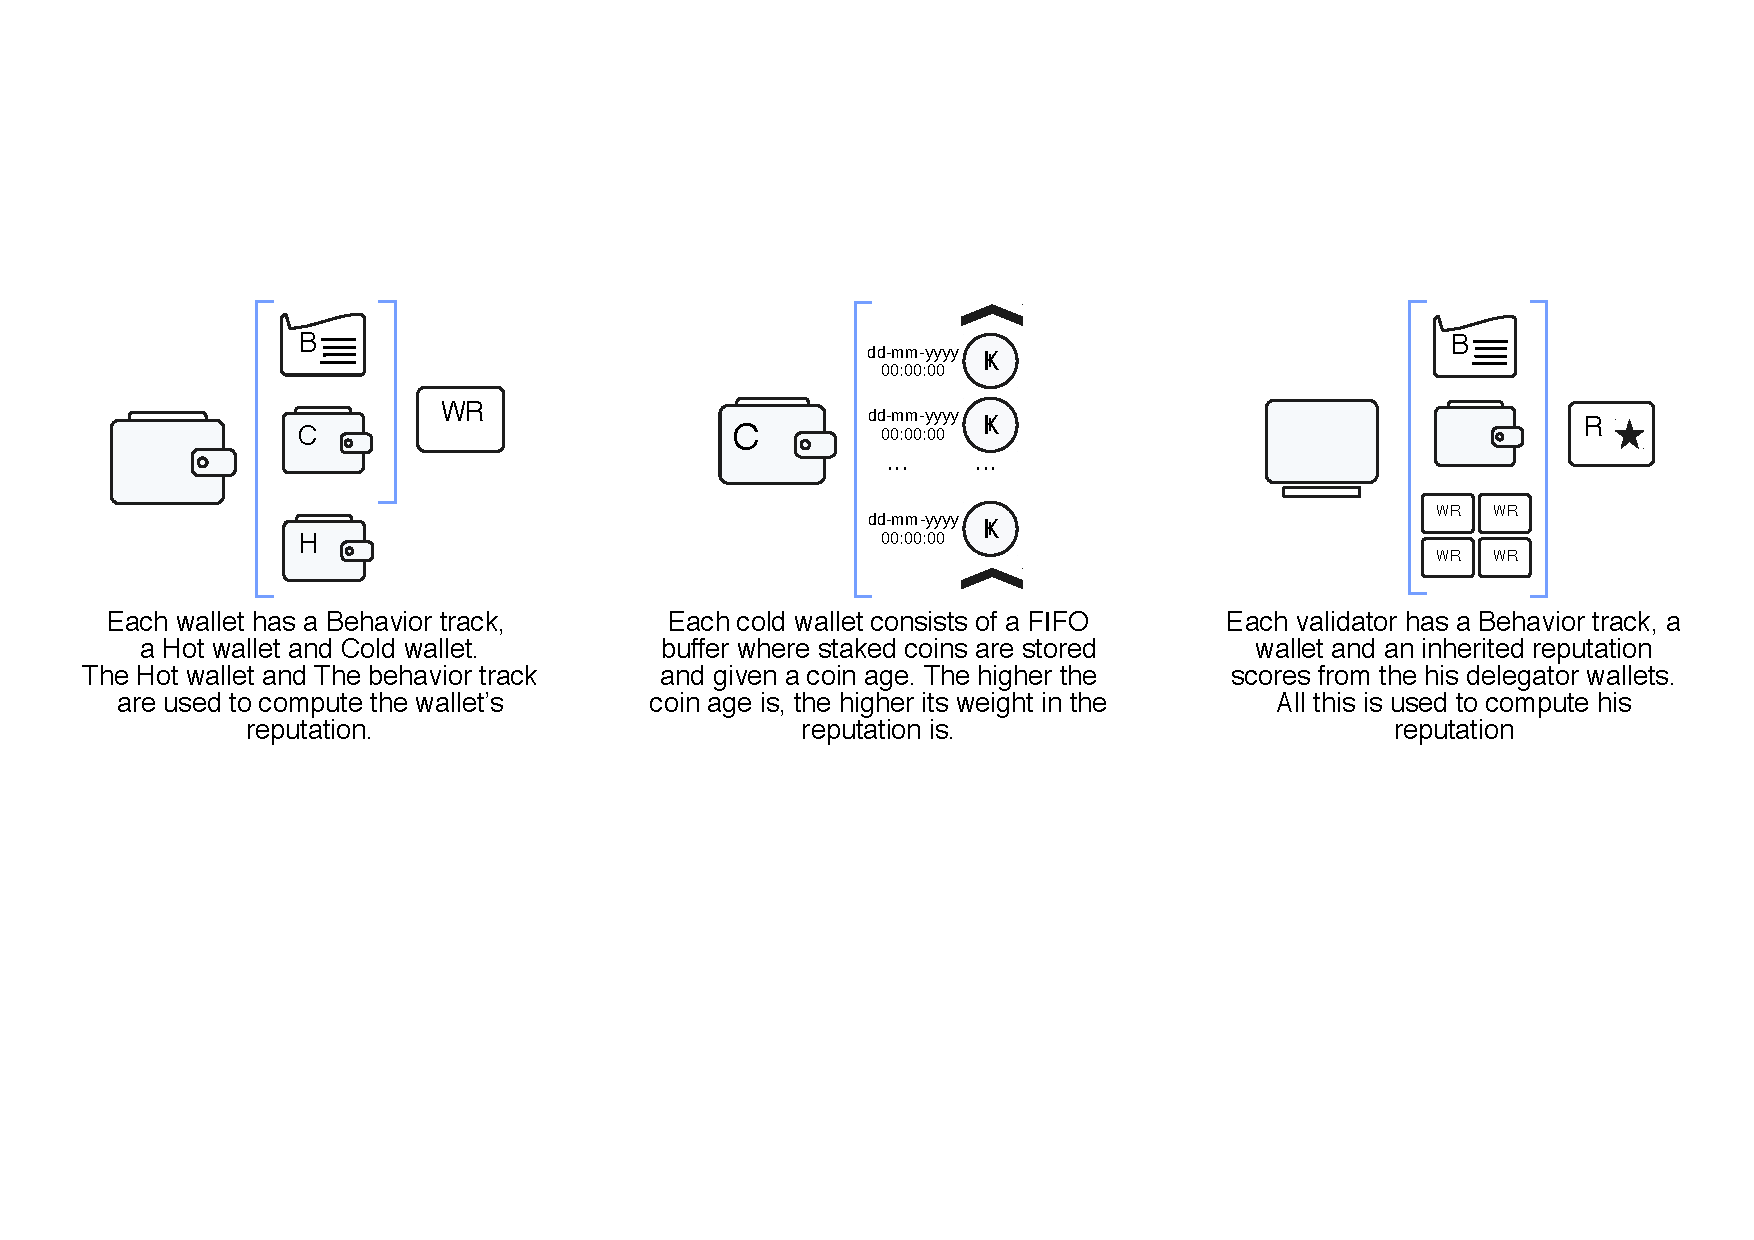
\includegraphics[width=\linewidth, trim= 1cm 8cm 1cm 5cm, clip]{Figures/wallets.pdf}
	\caption{The wallet structure and attributes in the Ki blockchain.}
	\label{fig:wallets}
\end{figure}

\textit{Using a cold wallet allows to improve the token liquidity while measuring the interest of the wallets in the ecosystem through their staked coin age and leveraging this interest in the reputation computation.}

\subsubsection{Dynamic Rewards} A tighter control of the number of yearly created tokens and relating it to the actual usage of the network are important factors in securing the value of the token. One extreme manner of achieving this value-centric control is to slash the reward for empty blocks since this only create an inflation that is not accompanied with a growth of interest in, and usage of, the token. While avoiding this "bad" inflation, zero reward for empty block can break the growth of the network by preventing the interest of the validator community, during the bootstrap. During this phase, empty blocks will constitute the vast majority of the validated blocks. If these blocks are not paid, validators will lose incentive since their ROI will be close to zero. Therefore, the reward function must involve both, a static and a dynamic reward factors. The first ensures that a minimum reward is paid regardless the payload of the block (at least during critical periods) and the second ensures that the number of created tokens is controlled and adjusted w.r.t. the goal yearly inflation rate.  
As mentioned earlier, minimal fixed reward should be paid for each block regardless the number of transactions it contains. In order to minimize the negative impact of this fixed reward when paid for empty blocks, its amount can be optimised by adapting it according to the ratio of empty blocks over the validated ones. Thus, fixed reward should be adjusted every period of time. Eventually this reward will tend to its minimal value \footnote{The static reward never reaches zero. A validator should be guaranteed a minimum payment regardless  the network state.} when this ratio drops below a given threshold. That is when the majority of validated blocks contains transactions, in which case paying for empty blocks is equivalent to creating negatively contributing tokens. The reward function must deal with the effect of projecting history based adjustment on the future for specific events such as sudden drop or sudden increase in transaction number. Moreover, the reward paid for an empty block must never be greater than a reward paid for a non-empty one. The dynamic part of the reward can be computed in two ways. On one hand, it can be computed on a block basis. That is, the yearly created tokens can be distributed over the number of blocks to be validated for the year. Since the number of validated blocks per year is an intrinsic parameter of the blockchain, this computation is deterministic. However, the limitation of the block based computation is its coarse granularity. That is, it occurs yearly and is independent from the number of transactions circulating on the network. The number of transactions is indeed the real indicator of the usage of the network and thus how viable it is. On the other hand, the dynamic part of the reward can be computed w.r.t. the number of transactions per year. That is, the reward paid per block is equal to the total rewards paid for the individual transactions contained in the block. In this case, the yearly created tokens are distributed over the number of transactions performed during the year. This allows for a more fine grained reward computation. The drawback here is that the number of transactions is not a configurable parameter of the blockchain, thus not deterministic. In other words, the dynamic reward here relies on not only, a yearly growth projection, but also the trend of this projection. Following are the details of this approach.  
\paragraph{Setup:} 
We start by defining the global constants of the environment. Let: 
\begin{itemize}
	\item $I$ be the number of created tokens for the year i.e. the inflation.
	\item $B$ be the number of validated blocks for the year.
	\item $T_{max}$ be the maximum number transactions that can be found in a block b.
\end{itemize}

Second we define the variables of the system. Let:
\begin{itemize}
	\item $t$ denote a transaction.
	\item $b$ denote a block.
	\item $R_b$ denote the reward paid for a block b.
	\item $T_b$ denote the transactions found in a block b.
	\item $\hat{T}$ denote the estimated number of transactions for the year.
	\item $\bar{T}_b$ denote the remaining transactions for the year after block b.
	\item $\bar{B}_b$ denote the remaining blocks for the year after block b.
\end{itemize}

Finally from the aforementioned constant and variables we derive the following: Let:
\begin{itemize}
	\item $f_b$ be the filling rate of a block:  $f_b=\frac{T_b}{T_{max}}$
	\item $sI$ be the static inflation and dI be the static inflation: $I=sI+dI$	
\end{itemize}

\paragraph{Reward computation :}
The main ideas of the proposal are described hereafter. The total reward to be paid per validated block is equal to the sum of two elements: a static element (sR) and a dynamic element (dR). That is : 
\begin{ceqn}
	\begin{align}
		R_b = sR_b +dR_b
	\end{align}
\end{ceqn}


Since the total amount of paid reward is fixed by the inflation for the current year, one has :
\begin{ceqn}
	\begin{align}
		\sum_{b=1}^{B}R_b=\sum_{b=1}^{B}(sR_b +dR_b) =sI + dI = I 
	\end{align}
\end{ceqn}

As mentioned earlier, the static part of the reward serves as incentive for the validators by  guaranteeing them a minimal payout base of their validation effort. Therefore it needs to be paid for each block regardless its payload and the moment at which it is validated. Accordingly, the static reward $sR_b$ given to a validator for validating a block is equal to :
\begin{ceqn}
	\begin{align}
		sR_b=\frac{sI}{B}
	\end{align}
\end{ceqn}

On its side, the second part of the reward i.e. the dynamic reward dRb adjusts the total reward according to the evolution of the network from a transaction point of view and guarantees the balance between a fair reward scheme and a controllable token creation. Indeed, if we assume that the total amount of created tokens for a given year is fix and predefined at the beginning of the year, then, at a given time point t, the amount of tokens that can be created and rewarded to the validator is equal to the remaining quota of created token for the year divided by the number of remaining blocks to be validated for the year. This is equivalent to distributing the dynamic reward over the blocks to be created in the years. Which first, renders the dynamic reward static and, second, does not take into account the evolution of the network from a transaction perspective. To tackle this problem we propose the following: first a theoretical dynamic Reward ($tdR$) is computed by distributing the dynamic inflation over the number of blocks. That is :
\begin{ceqn}
	\begin{align}
		tdR_b=\frac{dI}{B}
	\end{align}
\end{ceqn}
Then, each block $b$ is paid a fraction of $dR_b$ computed proportionally to the filling rate $f_b$ (see Section "Setup") of this block. That is : 
\begin{ceqn}
	\begin{align}
		dR_b=f_b \times tdR_b
	\end{align}
\end{ceqn}
Indeed, unless the filling rate is equal to 1 (that is when the block is full), a part of the theoretical reward, which we denote $\bar{dR}_b$, is not spent. It can be expressed as follows : 
\begin{ceqn}
	\begin{align}
		\bar{dR}_b=td_R - tdR_b
	\end{align}
\end{ceqn}
Here, one can act in two different manners : (i) $\bar{dR}_b$ is dropped from the inflation computation or (ii) $\bar{dR}_b$ is redistributed. In the next paragraphs these two strategies are explained and discussed.

$\bar{dR}_b$ is left over and only the tokens needed to reward the block w.r.t. its filling rate (Eq. 5) are created. On the one hand, this allows to to minimize the inflation by only paying the actual transactions. On the other hand, this might be non-incentivizing to the validators in the early phases of the blockchain life. Indeed, the block filling rates are very low during these periods which means that dynamic rewards might be extremely low.

$\bar{dR}_b$ is created (partially or entirely) and redistributed over the remaining blocks. By redistributing the remaining part of $tR_b$, one adjusts the dynamic reward w.r.t. the actual usage of the network solving consequently the low filling rate problem. The counterpart of  this strategy is that the resulting inflation is less faithful to the actual usage of the network. While not optimal, this still a better choice for the network vitality as it retains the validators' interest. Therefore, we adopt this strategy and formalize it as follows. The amount of KIs awarded to a validator for validating a block is equal to : 
\begin{ceqn}
	\begin{align}
		dR_b=f_b  \times ( tdR_b + \frac{I}{B-b} \sum_{j=0}^{b} \alpha \times \bar{dR}_j)
	\end{align}
\end{ceqn}
This formula can be expressed with the following words. At each block, the payable amount for a full block is increased by distributing the transferred reward from the previous unfilled blocks over the remaining block to be validated during the year. The paid amount is proportional to the the filling rate of the block. Note that ɑ is a hyperparameter that determine the transferable portion of the unpaid reward. 
While adapting the reward to the actual transaction load on the network, the strategy explained earlier might result in the accumulation of the dynamic reward on the last blocks of the year. In other words, validating a block at the end of the year will, unjustifiably,  be awarded with a large number of tokens. Which is not ideal. Practically, this might be caused by the low filling rate at the network launch which translates into a large amount of transferred rewards.  To counterbalance this, we propose to use the real filling rate, which we denote $f_b$ , instead of the theoretical filling rate. $f_b$ is continuously updated every $x$ blocks by using the last $x$ blocks to forecast the load for the upcoming $x$ blocks. The following parameters need to be determined : 

\begin{itemize}
	\item The update frequency determined by $x$.
	\item The forecasting function. 
\end{itemize}

\textit{Adapting the reward per validating block to the usage of the network allows to master the inflation and consequently, to maintain the value of the token.}

To demonstrate the impact of the forecasting function on the computation of the reward function we run an experimental study which we detail in this paragraph. The simulation has been run on the Ki simulator which is described further in this document. We considered the Bitcoin network as a real life source of data to simulate a realistic evolution of the transaction number and transaction distribution over the validated blocks during 10 years ([2009-2018]). We set the yearly inflation rate to 5\% and the static reward split to 20\% of the total inflation. That is equivalent to 1\% of the total supply. For the clarity purpose  we separately computed the total inflation rate achieved for each year using 6 naive forecasting models. These are shown in Table \ref{tab:forecast}. The reference period, i.e. the number of historical block used to predict the practical maximum number of transaction for the upcoming period has been fixed to 144 block. This is equivalent to 1 day. Consequently, the frequency of updating the practical maximum is once a day.

\begin{table}
	\footnotesize
	\begin{tabular}{|l | l|} 
		\hline
		Method & Description \\ [0.5ex] 
		\hline\hline
		Theoretical Max & The maximum number of tx per block fixed by the network\\ 
		\hline
		Prac. Max, Mean & The average number of tx per block over the reference period  \\
		\hline
		Prac. Max, 2 x Mean & Twice the average number of tx per block over the reference period \\
		\hline
		Prac. Max, Max & The maximum number of tx per block over the reference period \\
		\hline
		Prac. Max, 2 x Max & Twice the maximum number of tx per block over the reference period \\
		\hline
		Prac. Max, Linear & A linear growth of transaction number per day. \\ 
		\hline
	\end{tabular}
		\caption{The used forecasting functions.}
\label{tab:forecast}
\end{table}

Figure \ref{fig:sim} shows the results of the experiments. The transaction growth (Avg. Yearly. Tx) over the 10 years period is also shown for reference. It is clear that the best way of following the actual transaction growth is to use the theoretical average. That is because the latter directly transcribes the actual usage of the network w.r.t. its theoretical capacity. However, the problem here is that at the bootstrap of the system, the blocks are almost empty hence, the filling rate is very low. Which means tat only the static reward would be payed. This is what occurs for the first year (2009) where the total payed reward is almost equal to 1\% i.e. the mere static reward. This can be discouraging for the validators especially if the theoretical maximum transaction per block is set to high values for scalability concerns. 
As explained earlier in this section, the practical maximum can solve this limitation. One can approximate this practical maximum by looking to the previous day transactions and assuming that the average or the maximum of the previous day approximate the average and maximum for the current day. The green and red curves show how these basic predictors behaves. Clearly, when the growth is subtle (i.e., from 2009 to 2012), these predictors succeed in reflecting this growth an in adapting the inflation rate accordingly. However, when the growth becomes more accentuated (i.e. starting 2012), one can see that the set maximum inflation rate is consistently reached. That is because, when the network grows drastically, the maximum or the average function lies practical maximum values that are way lower than the reality causing the filling rate to reach one an the complete reward to be paid regardless the actual payload of the blocks. Amplifying these function by a certain factor (e.g., a factor of 2 in this experiments) helps solving this problem as shown by the orange curve. Yet, this is a data dependent result and a more generic predictor needs to be used.

\begin{figure}[h]
	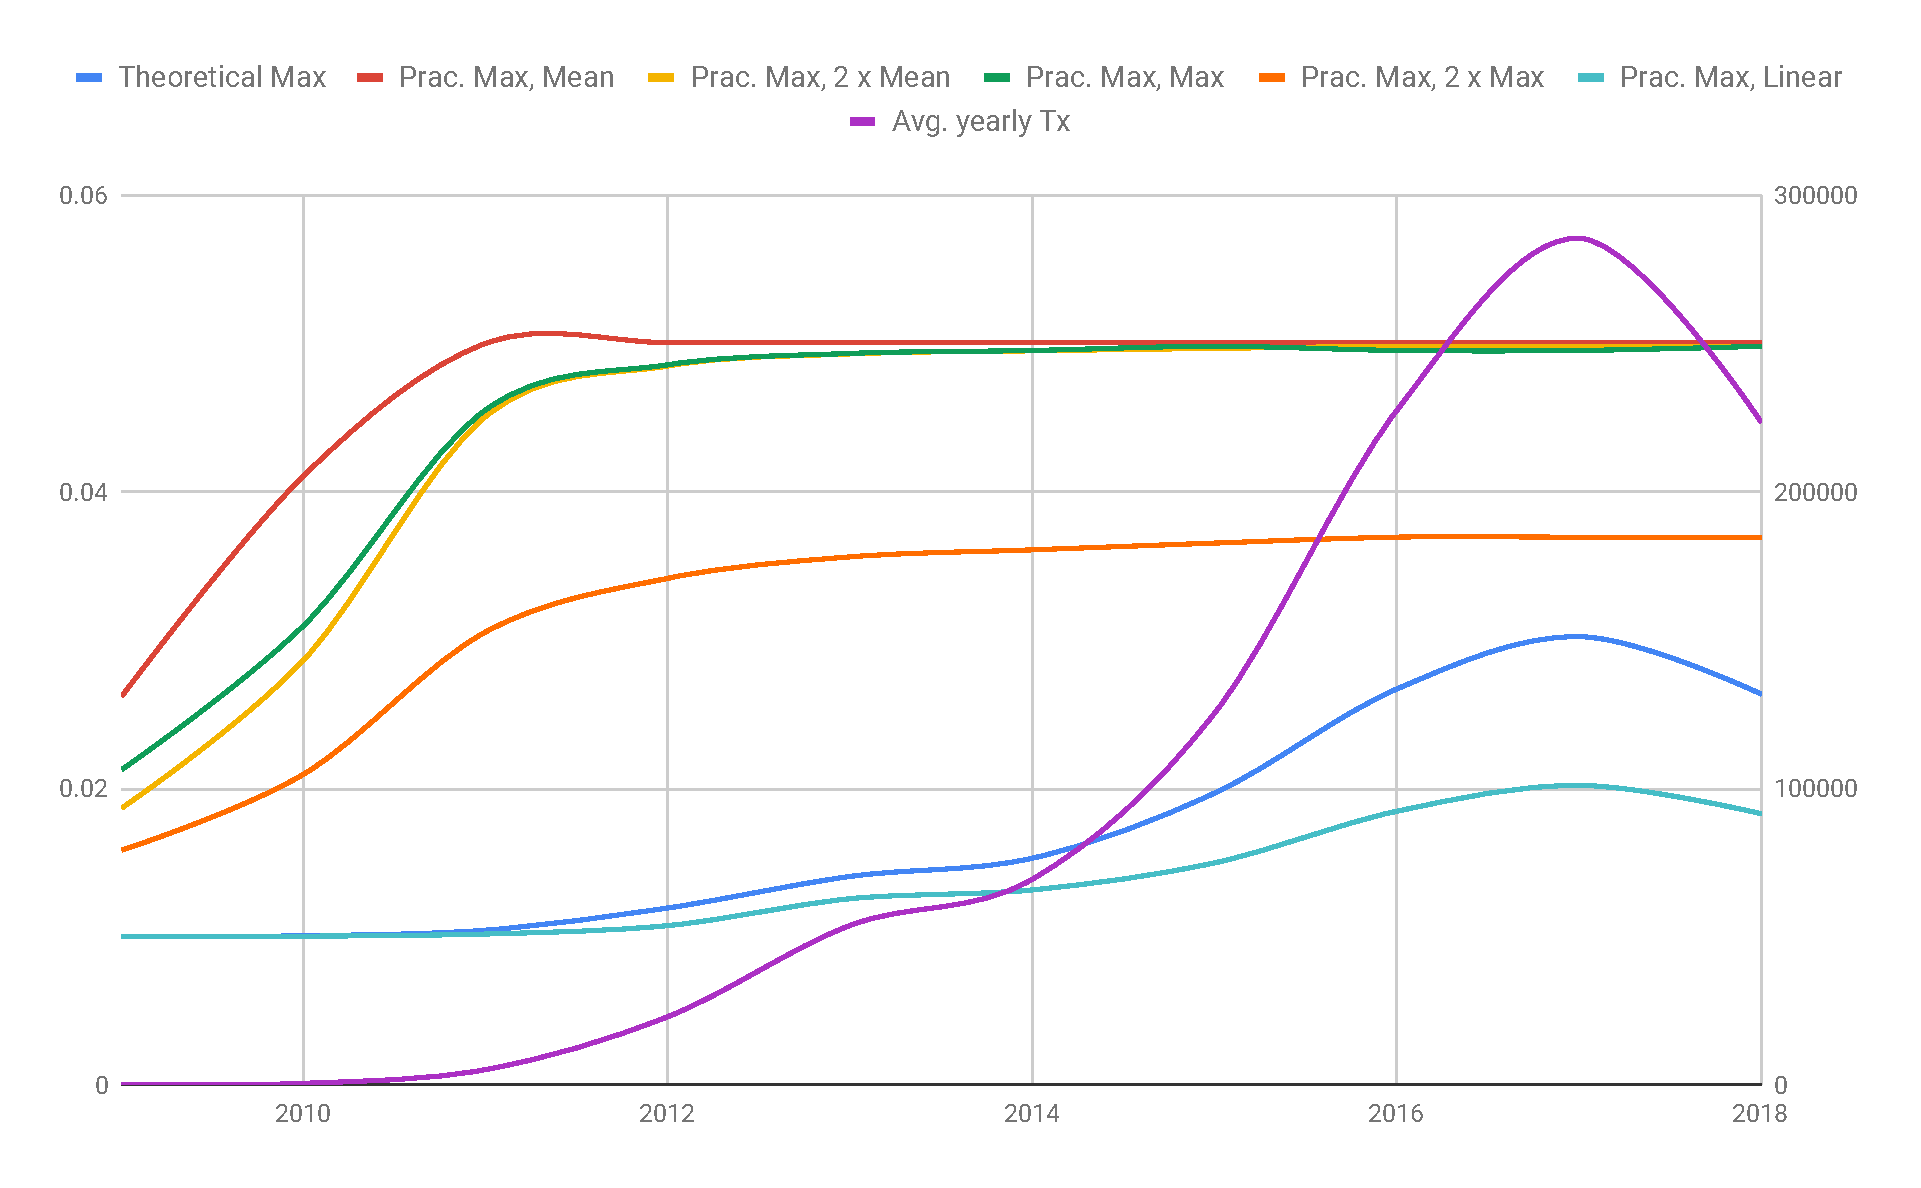
\includegraphics[width=\linewidth, trim= 0cm 0cm 0cm 0cm, clip]{Figures/exp.pdf}
	\caption{The reward growth over 10 years w.r.t. different forecasting methods.}
	\label{fig:sim}
\end{figure}

It is clear, according to the random walk theory, that it is impossible to accurately predict the evolution of the transaction numbers, hence of the practical maximum. Nonetheless, our goal is not to perform an accurate estimation but a rough upper bound estimation that allows a fair realistic reward and a resiliency to the sudden evolution that can be caused by market factors or intended attack (e.g. maxing out the blocks payload). Tuning both the update frequency and the forecasting function are needed to accomplish this goal.

\subsubsection{User privacy}
In the context of blockchain, one might identify two facets of the node privacy. The first relates to the transactions, that is who initiated a transaction and to whom is it destined. Indeed preserving the privacy of the nodes from the transaction perspective can emerge as a need for specific users in the ecosystem such as service providers who might want to hide their earnings from the public. The literature presents a fair amount of strategies that can address this concern with a minimal compromise on the performance and integrity levels. We specifically aim at using two techniques that have been used in other projects such as DUSK. These are the stealth addresses to protect transaction recipient anonymity and the Ring signature to protect transaction sender’s identity.

The second privacy facet relates to the information needed to trust a node. That is to the information required by the PoR to compute the reputation score of a node. To address this challenge, we consider using nodes' behavior and data publicly available on the network such as it's latency, uptime, forks and so on. 

\subsection{Ki blockchain tools}
multiple tools related to the deployment and improvement of the KI blockchain have been already made available by Genki’s team. Other tools will be available very soon. We summarize them as follows: 
\paragraph{Ki Devnet: }At the end of December 2018, we deployed the KI development network (codename: MizuKI) in order to allow testing the gradual improvement that will be made on the various levels cited earlier. It is possible for anyone to install and run a devnet relay and validator by following simple steps that can be found at: \url{https://github.com/KiFoundation/ki-deployer}. The KI Devnet launched with : 
\begin{itemize}
\item 3 seed servers 
\item 51 genesis validators 
\item 5 relays 
\item 5 real validators. 
\item 800 million DҜ. 
\end{itemize}

MizuKI is based on the 2nd version of the ARK core blockchain. The ARK ecosystem provides a complete tool bundle that allows to quickly deploy a DPoS based blockchain and to easily configure and use its subjacent tools such as the explorer and the wallets. All this is continuously maintained and improved by a active team and an engaged community. The Ki blockchain uses a fork of the ARK code, in which the DPoS protocol will be substituted by the PoR and other functionality such as the rewarding strategies and the wallet scheme will be added. 

\paragraph{Ki Explorer:} Transactions, blocks, wallets and validators can be monitored on the KI explorer of which the interface is shown in Figure \ref{fig:explorer}. It is available at: \url{http://blockchain.ki/}

\begin{figure}
	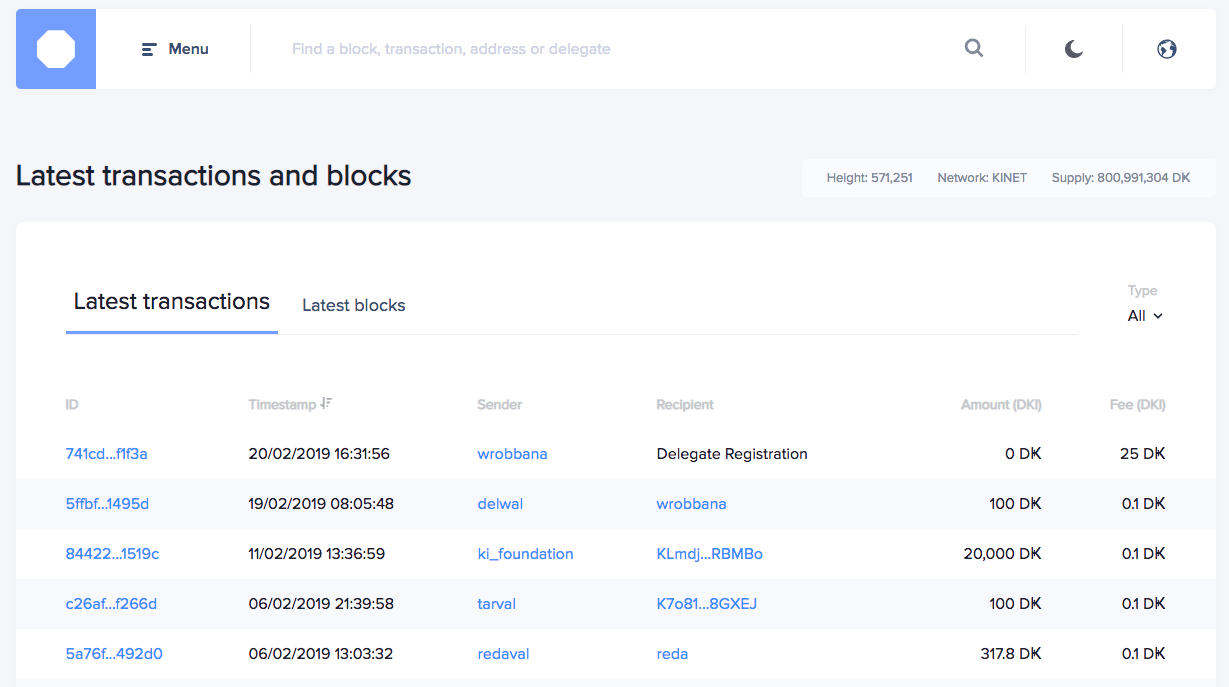
\includegraphics[width=\linewidth, trim= 0cm 0cm 0cm 0cm, clip]{Figures/explorer1}
	\caption{The Ki explorer user interface.}
	\label{fig:explorer}
\end{figure}

\paragraph{Ki wallets:} Starting January 2019, the code for building the Ki mobile wallet is available online. A downloadable version is also available on both the Google Play Store and the Apple Application Store. The wallets allows to receive and transfer KI tokens (or DKI tokens on the Devnet) as well as to register validators. Multiple views of the mobile wallet interface can be shown in Figure \ref{fig:walletapp}. The source code of the mobile wallet can be accessed on Github at: \url{https://github.com/KiFoundation/mobile-wallet}
\begin{figure}
	
\includegraphics[width=0.32\linewidth, trim= 0cm 0cm 0cm 0cm, clip]{Figures/mw1}
	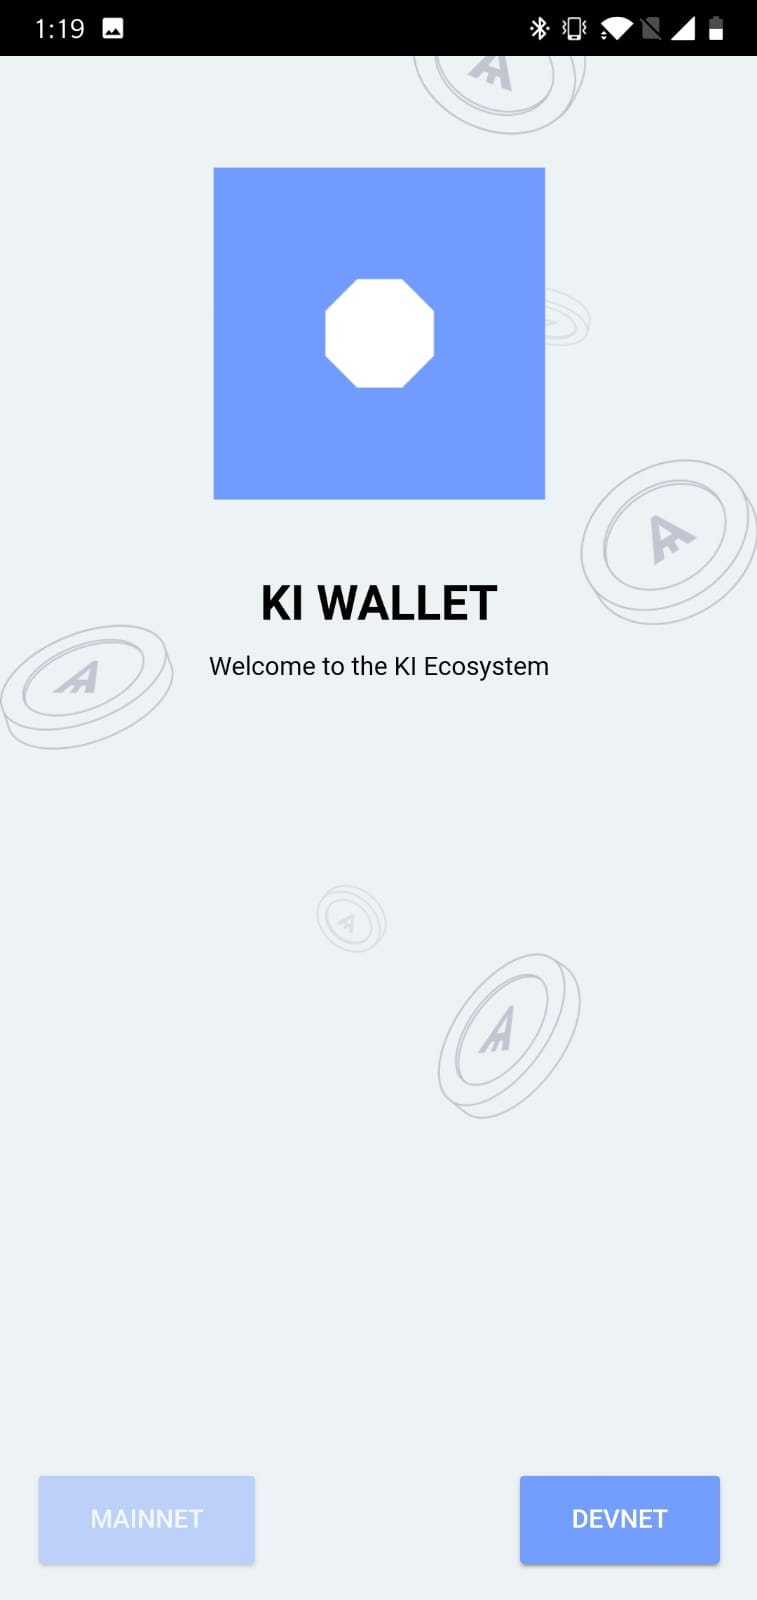
\includegraphics[width=0.32\linewidth, trim= 0cm 0cm 0cm 0cm, clip]{Figures/mw2}
	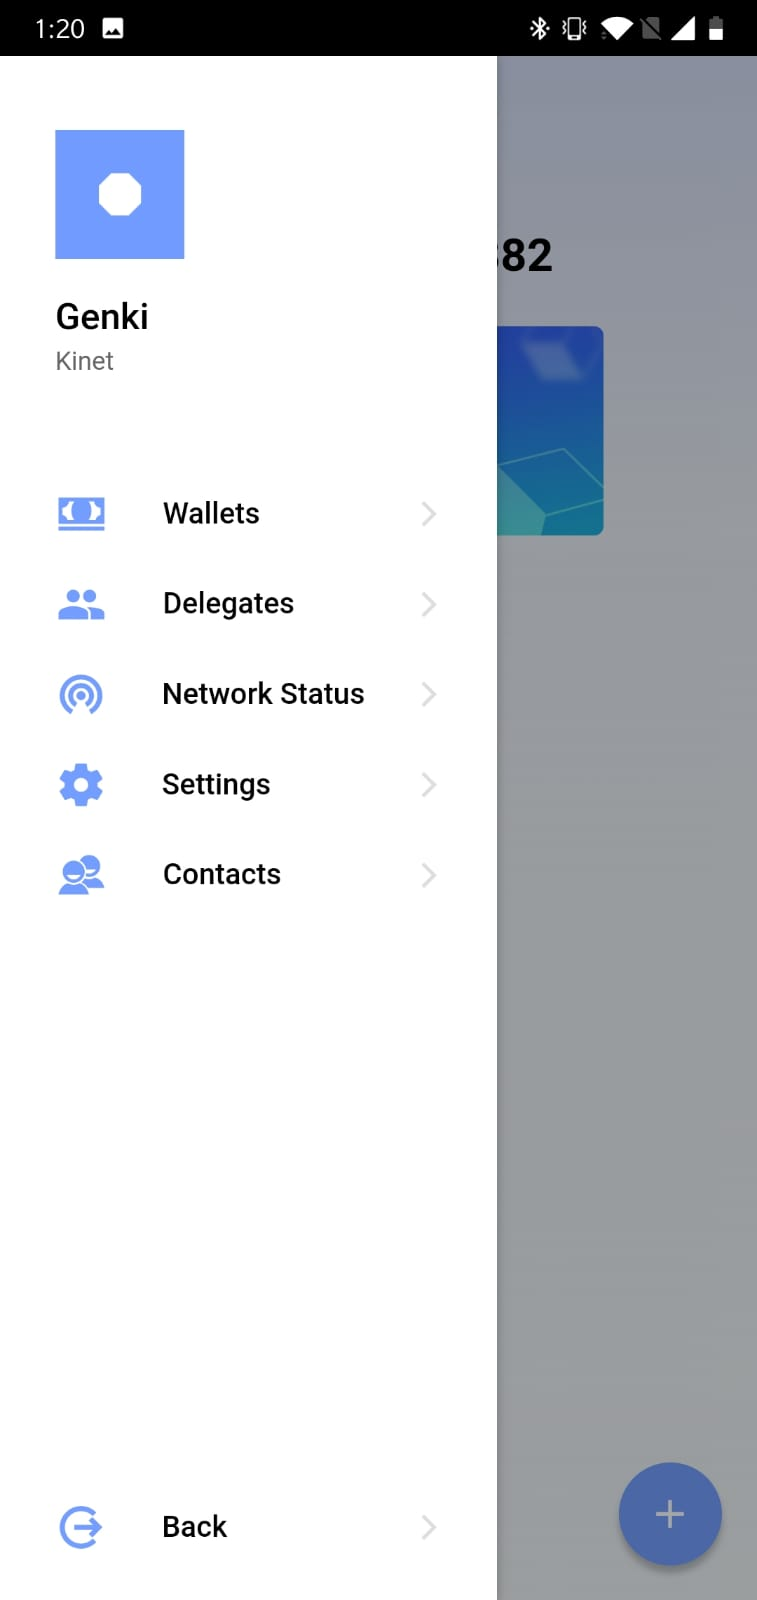
\includegraphics[width=0.32\linewidth, trim= 0cm 0cm 0cm 0cm, clip]{Figures/mw3}
	\caption{The Ki explorer user interface.}
	\label{fig:walletapp}
\end{figure}
\paragraph{Ki simulator:} In contrast with other distributed and peer to peer system for which well known simulators exist (e.g., PeerSim\footnote{http://peersim.sourceforge.net/}), there is no simulator adapted to blockchain networks and their scenarios. The Ki foundation plans to accompany the development of the Ki blockchain by the iterative release of the Ki simulator. The Ki simulator aims at giving a better idea on the throughput, stability and security of the network with respect to the protocol parameters such as the number of validators, their behavior, the number of transactions, the reputation measures, and so on. It allows to simulate situations which are not-and must not be-easily reproducible in real life. The planned iteration of the simulator will include the following components\footnote{The Ki Simulator can be accessed on github at: \url{https://github.com/KiFoundation/ki-simulator}}:

\begin{description}
	\item[Reward Simulator] The reward simulator aims at evaluating and comparing the stability and consistency of different dynamic and static rewarding schemes on real and synthetic data.
	\item[Reputation Simulator] The reputation simulator aims at testing the coverage of the behavior aggregation function explained earlier w.r.t. the workers' behaviors modeled through configurable scenarios. We plan to build a configuration layer on top of the RACOON simulator\footnote{A Framework for the Design Configuration of Accountable Selfish-Resilient Peer-to-Peer Systems \url{https://hal.inria.fr/hal-01250717/file/racoon-master.pdf}} to extend its support to blockchain related selfish and malicious behavior.
	\item[Performance simulator] The performance simulator aims at evaluating the scalability of the blockchain from the throughput (tx/sec) perspective. This is to study the impact of the validator list unlimited size, the random selection and the reputation computation on the network performance.
\end{description}
 
To date, a prototype of the reward simulator has been implemented in Python. The current version is constituted by the following modules: 
\begin{description}
	\item[The data generator] It allows to load and format transaction data from a data file, to generate transaction data from a preset distribution configuration, to generate a set of validators with their relative stakes from a preset distribution configuration and to distribute the validation spots over the generated validators based on a preset strategy.
	\item[The forecasting module] It allows to make predictions on the number of transaction based on historical data based on known models such as the "Autoregressive integrated moving average" (ARIMA).
	\item[The reward calculator] It allows to compute the reward based on 4 models : (i) transaction based reward, (ii) block based reward, (iii) hybrid reward and (iv) transfer based reward (Ki's model). Besides, it allows to compute the individual reward of each validator based on their validation spots.
\end{description}


\subsection{Ki blockchain roadmap}
\begin{figure}[h]
	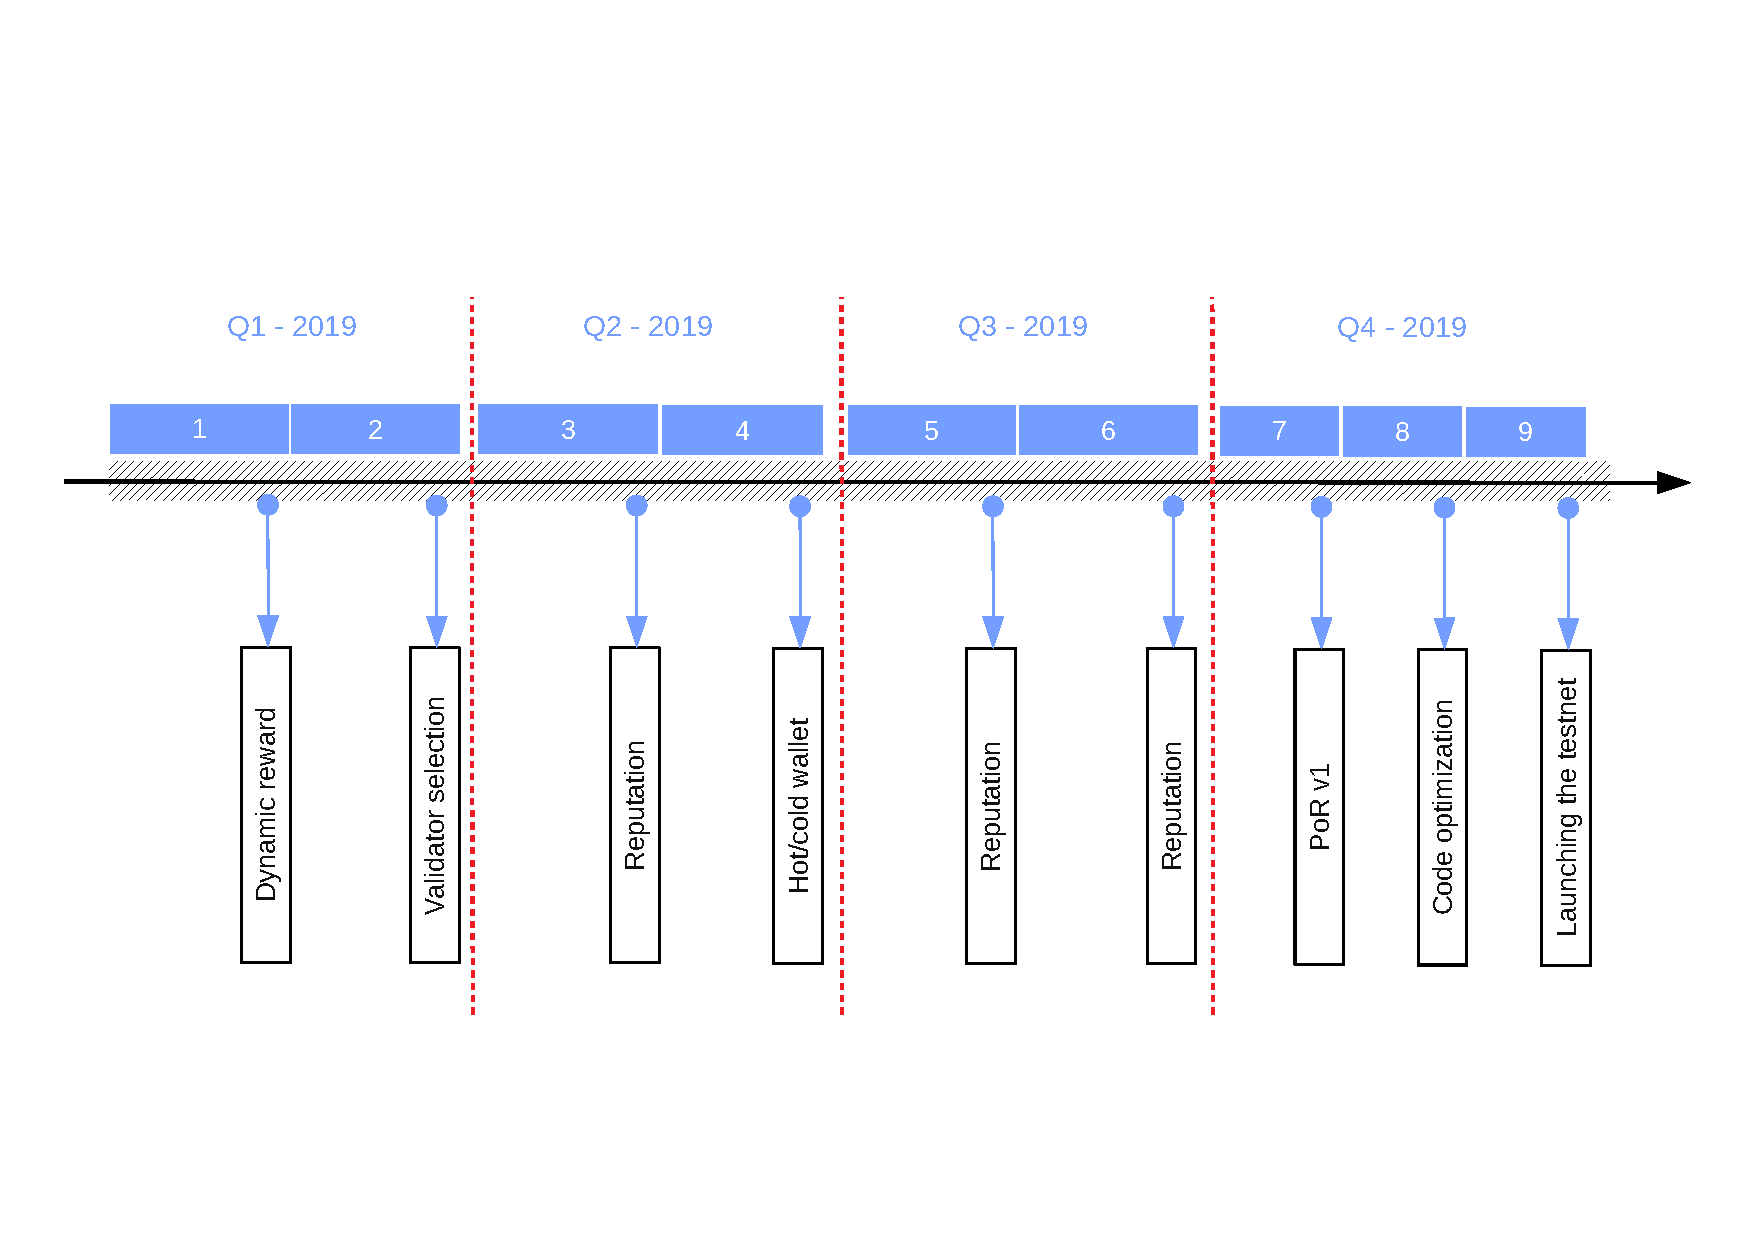
\includegraphics[width=\linewidth, trim= 1cm 3cm 1cm 3.5cm, clip]{Figures/Roadmap_f.pdf}
	\caption{An overview on the research and implementation roadmap of the Ki blockchain.}
	\label{fig:roadmap}
\end{figure}

It is clear from the previous discussions that the challenges are dependent one on another. Moreover, it is clear that besides the needed implementation and development effort, an upstream theoretical effort is mandatory. This dependency and challenging research aspects implies a gradual and interlaced work. That is, at each milestone we will be fixing, as much as it is logically possible, all the elements except the one we are dealing with at that moment. The roadmap in Figure \ref{fig:roadmap} depicts this process and shows how the task will be distributed over the upcoming year, with the ultimate goal being to launch a Testnet that fully supports the PoR consensus protocol by the end of December 2019.

\section{The Ki device, A smartspeaker and IoT master, the bootstrap of the Ki Ecosystem}
Ki’s homepod enables owners of untapped IT assets to monetise their space capacity, in a similar way to how AirBnB enables homeowners to monetise spare rooms within their own households. The Ki device exists to protect its owner’s digital sovereignty, while allowing them to monetise their untapped digital assets. 
On a larger scale, the Ki device can be seen not only as the hub of a smart home ecosystem, but also as a core component of tomorrow's smart city, managing its inhabitants’ IT assets as cleverly as a smart grid can manage a city’s energy [3].
To achieve such a vision, Ki need to address different challenges:
\begin{itemize}
	\item Unify heterogeneous wireless communication technologies, to make Ki’s Homepod a hub to all the digital assets located on its owner’s local area network.
	\item Give true digital sovereignty to its owner over their LAN, by letting them monetise their IT assets as they wish, without any central control, not even Ki’s.
	\item Ensure the end user’s privacy.
\end{itemize}

Addressing these issues in a comprehensive and effective way led us to create the Ki device: a smartspeaker that’s also a powerful network hub, which includes all the needed components and software to communicate wirelessly, manage applications, and share resources, while ensuring security and privacy for its users. 

\begin{figure}
	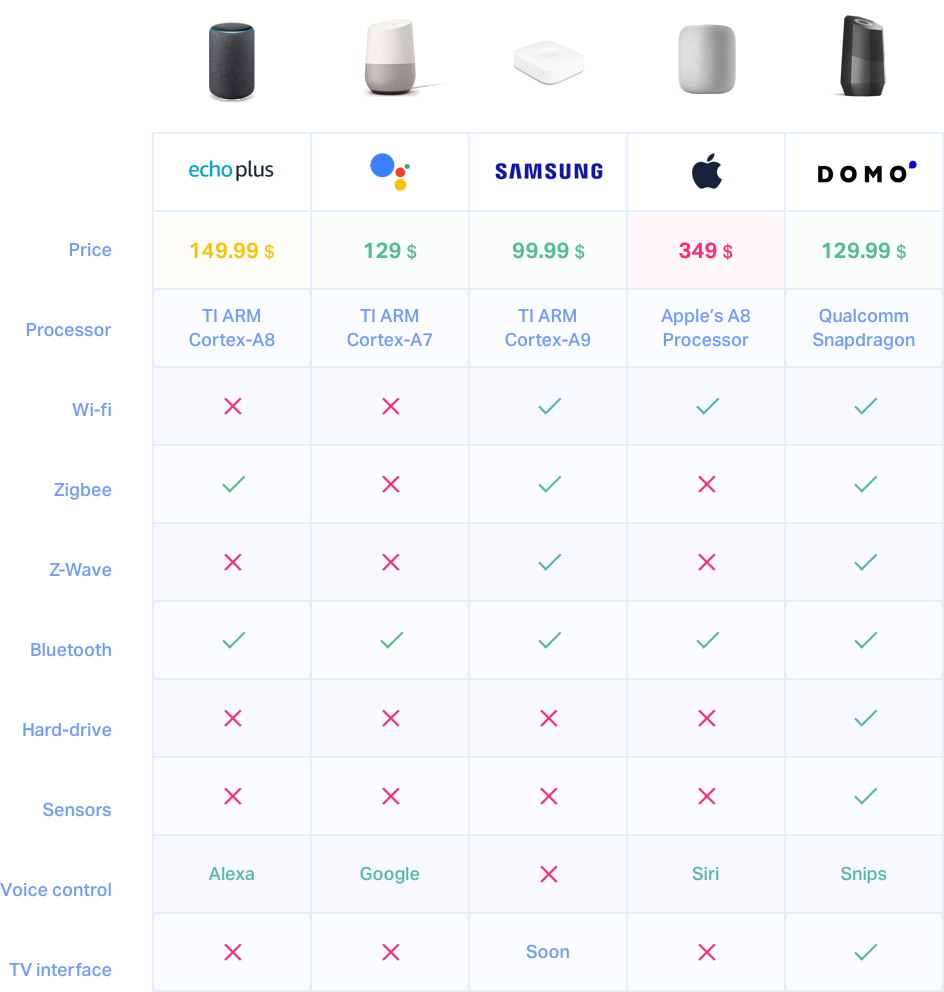
\includegraphics[width=\linewidth, trim= 0cm 0cm 0cm 0cm, clip]{Figures/domoD.png}
	\caption{Smart speaker competition scorecard.}
	\label{fig:domoD}
\end{figure}

\subsection{A privacy-first approach}
A privacy-centric approach drives the integration of privacy friendly technologies in the Ki device, such as its voice platform that runs locally, ensuring that its users’ conversations aren’t uploaded to a cloud-based system.  This means that they remain private at all times. Ki’s users’ voices, which are a critical biometric footprint, are not shared with anybody. 
Every technology built for the Ki network is done in a “privacy-by-design” approach, and every algorithm that uses user data, runs locally and securely. Privacy is a fundamental part of Ki’s approach to building a smart speaker: we consider it a fundamental right.
Other smart home devices are simply a speaker and a microphone. They cannot support a network or decentralised internet. The Ki Foundation has built a home device that utilises a new Operating System based on AOSP holding libraries supporting Blockchain-based and decentralized application store (the dApp Store). Both of which can never be leveraged to listen, manipulate or monetise its occupants personal data. The Ki home device is the first decentralised, privacy-first IoT hub that acts as a gatekeeper of your personal and private data, wherever you call home. Unlike existing smartspeaker devices, that simply have a microphone and a speaker, Ki’s device (fig. below) is a real computer, equipped with powerful processors, an SSD storage and multiple sensors. As such, every Ki device can be a setup as a validator node in the Ki blockchain, contributing to the operation, maintenance and governance of its ecosystem. The Ki device is equipped with a loud speaker, audio devices that never transmit data out of the home and further, is equipped with smart sensors that can track energy usage, temperature, air quality and humidity. The Ki provides Wifi internet through 2 different channels: 1)  an Ethernet plug, or 2) eSIM solution service that enables data traffic in more than 200 destinations in the world. The eSIM provides a fallback connectivity solution in case the landline internet is cut.

\begin{figure}
	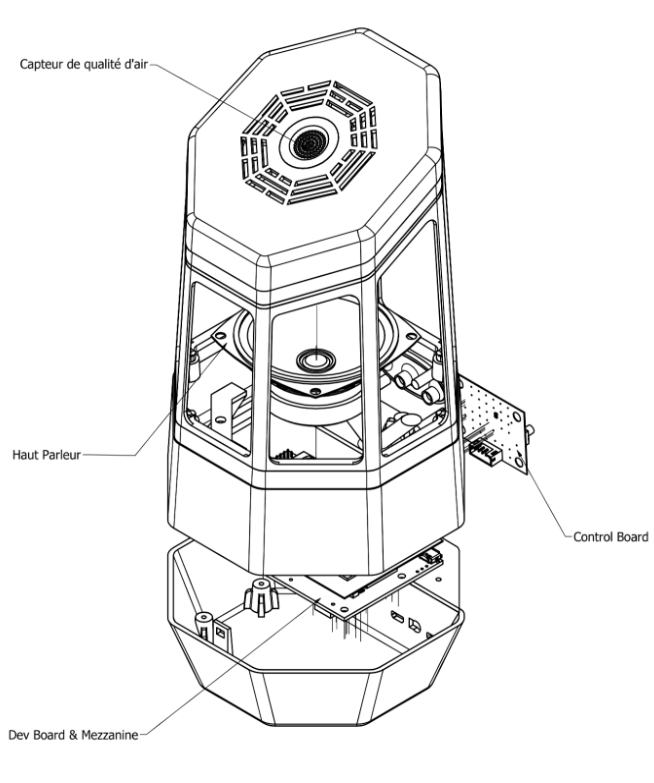
\includegraphics[width=0.49\linewidth, trim= 0cm 0cm 0cm 0cm, clip]{Figures/domoE.png}
	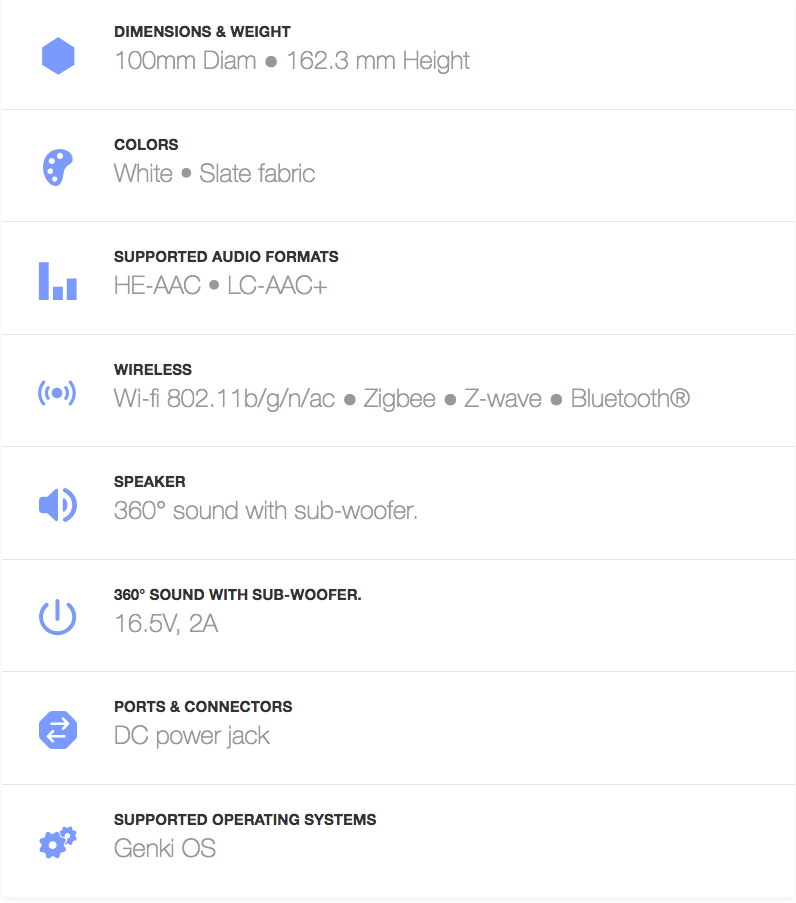
\includegraphics[width=0.49\linewidth, trim= 0cm 0cm 0cm 0cm, clip]{Figures/domoS.png}
	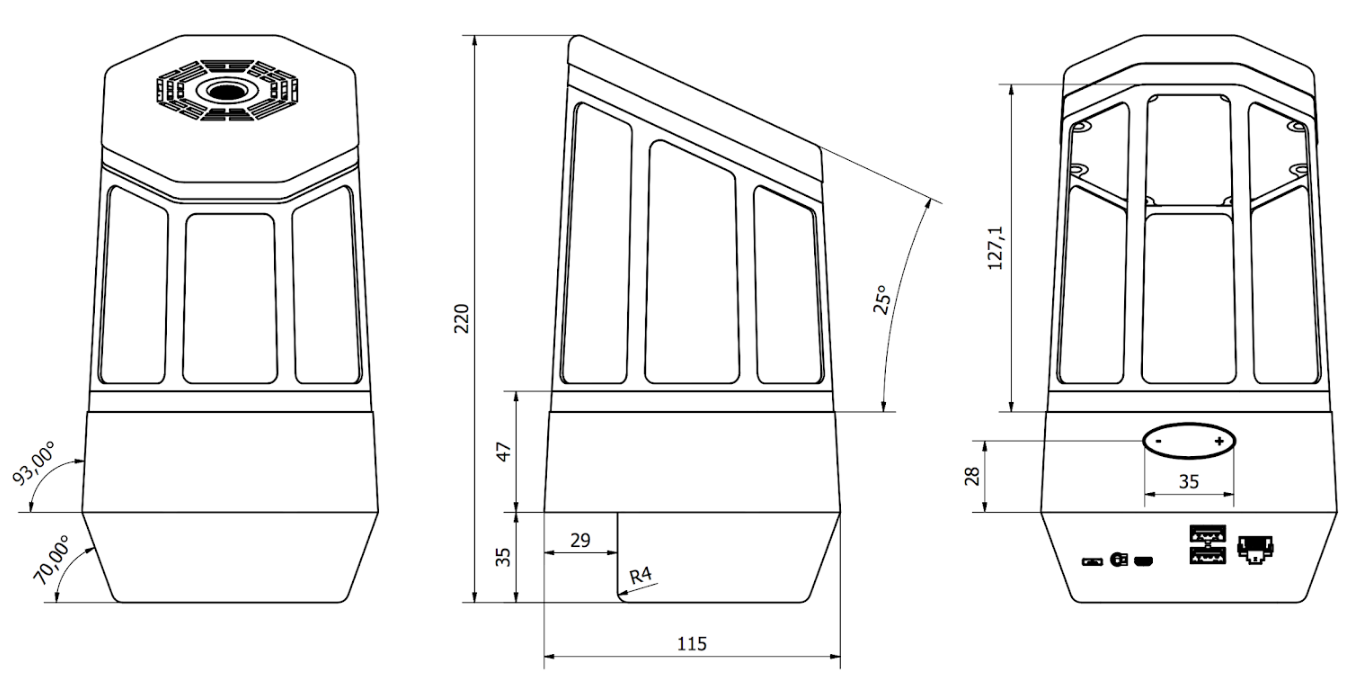
\includegraphics[width=\linewidth, trim= 0cm 0cm 0cm 0cm, clip]{Figures/domoB.png}
	\caption{The Ki device specifications.}
	\label{fig:domo}
\end{figure}

\subsection{Building resiliency and security}
Relying on a centralised cloud-based technology to operate your home will inevitably run into the “single point of failure” problem [8], if not a temporary disruption of your internet access, making your connected home useless. With Ki, users do not rely on a unique service provider to benefit from the service and users therefore become resilient to such severance. 

\section{The Ki ecosystem }
\subsection{Stakeholders}
The Ki ecosystem is made up of 3 kind of players, each with a distinct role in the proper and efficient functioning of the network.
\paragraph{Validators}
A validator is a fully synchronised node, willing to stake its tokens or part of its tokens to secure the network (i.e., willing to participate in the consensus protocol). A validator is paid in Ki tokens for their participation. These validators contribute to the consensus by broadcasting votes cryptographically signed by each validator, using their private key.
Validator candidates can stake their own Ki tokens or have tokens "delegated" to them by delegators. The Ki Blockchain can have an unlimited number of validator candidates due to its PoR consensus algorithm.
Validators and their delegators will earn a dynamic amount of Ki tokens, depending on the number of daily transactions witnessed on the system. There will never be any transaction fees on the network, although a validator will be able to charge a commission on the tokens forwarded to their delegators as an incentive for running a full node. 
If a validator misbehaves, its reputation is affected, and its staked Ki tokens (including delegated tokens) can be slashed. The penalty depends on the severity of the violation.
\paragraph{Delegators}
A delegator is a node that does not synchronise the full blockchain, but which lends part of its stake to help a validator increase its stake; the validator then redistributes the corresponding share of its reward to the delegator.
In this way, a delegator can also take part in securing the network and be rewarded proportionally to the amount of tokens they are willing to stake. If a validator’s stake is slashed due to an invalid behavior, the delegator share of the stake is slashed as well. As a result, the delegator shares this risk and must delegate wisely.

\paragraph{Service providers and developers}
By requiring apps to be installed through App Stores, under the control of those managing the operating systems, a choke point was created. Since most people rely on Apple or Android operating systems for their devices, these companies have gained huge leverage on the flows of information.
The Ki ecosystem is underpinned by the Ki Blockchain and bootstrapped by the Ki device will have the dApp Store at its core. This is an open platform where third-party software developers can reach new markets, and use decentralised resources to offer innovative services: securely, fairly and reliably. By embracing decentralisation, developers won’t need a third party to manage transactions, avoiding transaction fees in the process. The dApp store will manage the reputations of the developers and service providers selling to consumers using certain of the techniques incorporated in the PoR algorithm. 
Governance of the dApp Store will eventually be completed delegated to the open source code developed by the Ki Foundation and the votes of the holders of Ki tokens. Certain stakes of Ki tokens will be required to sell services and develop applications for sale in the dApp Store. 
A service provider can rent its unused resources (e.g. hardware or bandwidth) through third party applications and get paid in Ki tokens for the resources they provide. Every Ki device owner will be able to enable or disable their devices ability to provide resources to the network and become a service provider. 
IoT fleet owners will also be able to join the network and offer their computational power, network and storage for Ki tokens. For example, public WiFi providers, connected hard drives owners, router manufacturers, etc. could all provide computing, storage \& validation services. End consumers may pay for storage and computation services using fiat currency, which is then converted into Ki tokens using the Blockchain Client Software layer, which determines the best rate to acquire Ki tokens and dispatches them to the service provider.

\paragraph{Device owners}
By acquiring a Ki, you can also become a full actor in the Ki Blockchain: by staking Kis as a validator and by providing the devices’ storage and processing power to maintain and secure the blockchain.
Device owners could earn approx \$15/month depending on how much computing power and storage their device commits to the Ki network or other decentralised networks and services. Every device owner will be able to enable or disable its ability to provide some service for the community. IoT fleet owners will also be able to join the network and offer their computational power, network and storage for Kis. Examples of other devices that could become part of the Ki ecosystem include: public WiFi providers, connected hard drives owners, router manufacturers, etc.

\subsection{Bringing wireless communications together}
Big tech companies have a natural tendency to impose proprietary protocols to enforce their monopoly. In the IoT emerging market, the same trend has been observed across all actors: from Amazon’s Zigbee rooting to Samsung’s z-wave rooting, and throughout other wireless technologies such as Sigfox and Lora.

This led us to create an agnostic technological layer, merging all systems and acting as a conductor, orchestrating all communications with a fully open protocol that shares value for all rather than extracting value for the few.

\begin{figure}
	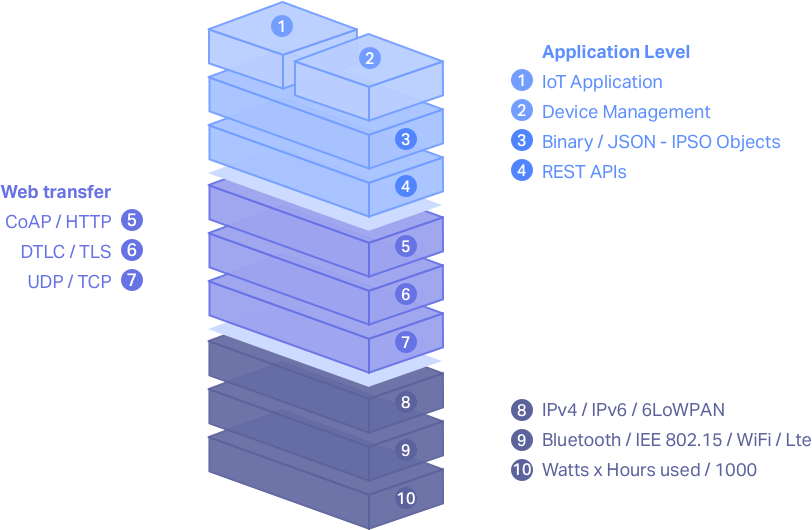
\includegraphics[width=\linewidth, trim= 0cm 0cm 0cm 0cm, clip]{Figures/iot.png}
	\caption{Layers of value and service in the IoT world.}
	\label{fig:iot}
\end{figure}

While the world is currently embracing various home connected hardware, their use and interaction is still limited to basic tasks, mostly due to a lack of a coherent layer unifying communication protocols, application stores and resilient services that is open to the broader software development community. The Ki device aims to become the cornerstone of a new internet, Web3.0. It is a decentralised infrastructure that provides the ability to deploy a truly decentralised, fair and transparent ecosystem.
\begin{figure}
	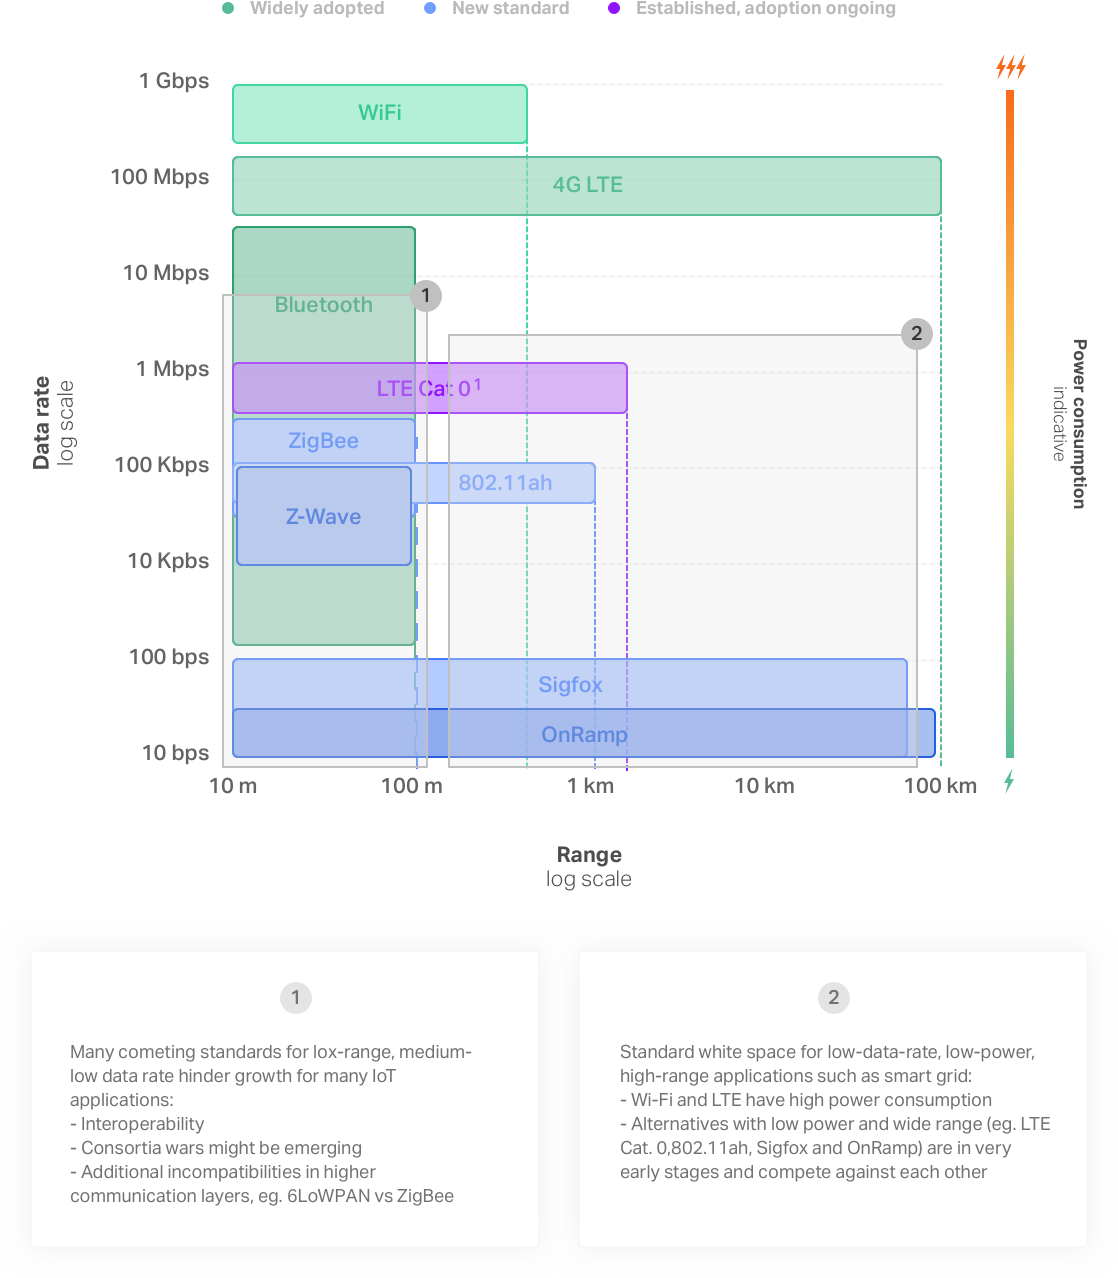
\includegraphics[width=\linewidth, trim= 0cm 0cm 0cm 0cm, clip]{Figures/wireless.png}
	\caption{Layers of value and service in the IoT world.}
	\label{fig:wireless}
\end{figure}
\subsection{Enabling a global decentralised mobile network}
With the explosive growth of IoT and other decentralised applications, we see a compelling need to support the process of local compute, store and communication. Getting closer to edges and also requiring real-time speeds, the conventional cloud model of having to rely on remote centralised computing resource is no longer feasible to support billions of things requiring near real-time latencies.

The Ki Foundation is partnering with OnOff to create the first decentralised mobile network. OnOff’s unique soft-switch technology [10] allows any smartphone with the OnOff App installed to seamlessly use the closest Ki mesh network for VoIP communication, and leverage the Ki Blockchain to pay for bandwidth usage. Each participating Ki device owner will receive Kis as payment for the used bandwidth.

Both through the internal technology and the way that partners can leverage technology within the Ki ecosystem, user privacy comes first. In Ki’s proposed new decentralised mobile network, public-private cryptography will be used to identify devices (such as  smartphones) and link them to a subscriber’s identity. Instead of requiring IMEI identification to connect a mobile phone to a Ki device to share VoIP bandwidth resources, the Ki Wallet will share a public key for broadcast instead. This public key is generated from the private key, which is stored securely on the device, with neither the carrier nor any other third party having access to it. 

Since each base station is a node of the Ki Blockchain, each device’s identity is readily available and can be authenticated quickly, by only sending its public key. Each Ki device can participate and support this mobile infrastructure and, therefore, can act as one of its nodes. Once a dense enough mesh network of Ki devices is established, they will together enable a new decentralised global wireless network.

\subsection{The Ki Token}

Within the Ki Network the native Ki token is used to facilitate all services and transactions on the network. It also provides the holder with the ability to validate, delegate to other validators and to vote on Ki network proposals. The Ki token forms a pivotal role in maintaining the security of the Ki Blockchain and rewarding validators for securing the network. 

The Ki token serves a number of roles within the Ki ecosystem:
\begin{itemize}
	\item As a unit of account within the Ki network
	\item As a means of transacting within the Ki Blockchain and Ki dApp store 
	\item As a means of transferring value for unused resources and third party services
	\item As a means of incentivising validators and delegators to secure the network
	\item As a means of transferring marketplace transaction fees in the Ki decentralised dApp store: all fees are shared among app developers and token holders participating as validators and delegators within the network
	\begin{itemize}
		\item Service providers receive 95% of all Ki spent in dApps on the Ki marketplace
		\item Validators and delegators receive 5% of all Ki spent  
	\end{itemize}
	\item As a means of measuring reputation within the Ki’s PoR consensus.
\end{itemize}


The Ki tokens’ initial supply has been set to 800 million tokens, but is not fixed. The Ki token has an inflationary policy to compensate validators through newly issued Ki tokens. Each Ki token held is time-stamped with the date of the holding, which provides its holder a higher validator weight the older the timestamp. Staked Ki tokens will also receive 5% of all fee rewards spent in the Ki marketplace in Ki, with the remaining 95% of Ki fee rewards being paid to service providers such as app developers or storage providers. 
In the Ki Network all value created by the network is directed back to token holders who actively participate in the network. By staking tokens, token holders capture value from the growth of transactions in the app store.
Token holders can participate in the early growth of the network by becoming validators or delegators to receive inflation rewards and marketplace fee share.

\subsection{Governance}

One of the most challenging things to get right in a decentralised system is governance. If we consider governance, “the process by which we attempt to establish (and maintain/revoke) the legitimacy of decisions, decision-making processes, and related governance norms/expectations,” we can conceive of many ways to establish the legitimacy of decisions. In some contexts, voting can play a critical role. In others, it’s not needed. However decisions affecting the network are made, they must make sure that all stakeholders are considered, and that no single stakeholder or organisation holds too much sway without checks and balances on that power or influence. 

While we believe that to give Ki the best chance of succeeding, there is a need to have control in the early days, such control will be carried out in consultation with a strong governance and advisory board of varied backgrounds and interests to represent the wider interests of the Ki network. Extensive governance protections will be implemented in the Ki ecosystem: the constitutional charter of the foundation and its governing and advisory boards as well as other mechanisms such as those that are “on chain” (via the Ki blockchain’s protocol) and informal “off chain” mechanisms (via the social structures around the Ki ecosystem). 

Governance of the dApp Store will also eventually be completely delegated to the open source code developed by the Ki Foundation and the votes of the holders of Ki tokens. The Ki Foundation will own the rights to the Ki device and the device will be used in furtherance of the Foundation’s mission: to create a new digital, connected home, built on a decentralised internet and the principles of privacy, security and the fair sharing of value. 

The end-goal is that Ki’s ecosystem will become completely decentralised, open source and governed on a decentralised basis by the community of Ki token holders. Governance is not a feature, it is a complex system and proper thought is being given to develop such a system for the Ki Foundation and ecosystem. A full governance white paper will be released prior to the launch of the Ki network.


